\documentclass[12pt]{exam}
\usepackage[margin=.6in,papersize={8.5in,17in}]{geometry}
\usepackage{enumitem}
\usepackage{tikz}
\usepackage{newtxtext,newtxmath}
\usepackage{bm}
\usepackage{siunitx}


\setlength{\parindent}{0pt}
\setlength{\headheight}{14pt}

\usetikzlibrary{patterns}

\pagestyle{headandfoot}
\header{}{}{}
\footer{}{}{}

\newcommand{\pic}[2]{
  \begin{center}
    \includegraphics[width=#1\textwidth]{#2}
  \end{center}
}

\sisetup{
  inter-unit-product =\ensuremath{\cdot{}},
  per-mode=symbol
}
\tikzset{
  >=latex
}


\renewcommand{\choiceshook}{
  \setlength{\leftmargin}{22pt}
  \setlength{\itemsep}{2pt}%.9\baselineskip}
  \setlength{\topsep}{0pt}
  \setlength\parsep{0pt}
}
\renewcommand{\choicelabel}{(\thechoice)}


\begin{document}

\begin{center}
  \textbf{AP AND IBHL PHYSICS PRACTICE TEST \#1\\
    PART 1: MULTIPLE-CHOICE QUESTIONS
  }
\end{center}

%\textbf{Directions:} Each of the questions or incomplete statements below is
%followed by five suggested answers or completions. Select the one that is best
%in each case and place the letter of your choice in the corresponding box on
%the student answer sheet.

\textbf{Questions \ref{proj1}--\ref{proj2}:} A 10 kg projectile is launched at
a \ang{60} angle to the ground with a velocity of \SI{200}{\metre\per\second}.
Neglect air resistance.

\begin{questions}
  
  \question Compare this projectile with a 5 kg projectile launched under the
  same conditions but at a \ang{30} angle. The 5 kg projectile will
  \label{proj1}
  \begin{choices}
    \choice go higher up and farther along the ground
    \choice go equally high and equally far along the ground
    \choice neither go as high nor as far along the ground
    \choice not go as high but go equally far along the ground
  \end{choices}
    
  \question As the launch angle is lowered to \ang{45}, the maximum horizontal
  distance traveled by the projectile will
  \label{proj2}
  \begin{choices}
    \choice decrease
    \choice increase
    \choice remain the same
    \choice be impossible to determine without more information
  \end{choices}

  \uplevel{
    \pic{.4}{IMG_20200810_093039201}
  }
  \question A car with a 500 N driver goes over a hill that has a radius of 50
  meters as shown in the figure above. The velocity of the car is
  \SI{20}{\metre\per\second}. What are the approximate force and direction
  that the car exerts on the driver?
  \begin{choices}
    \choice\SI{900}{\newton}, up
    \choice\SI{400}{\newton}, down
    \choice\SI{100}{\newton}, up
    \choice\SI{500}{\newton}, up
  \end{choices}
  
  \uplevel{
    \pic{.27}{falling-blocks}
  }
  \question Block $Y$ with mass $m_Y$ falls onto and sticks to block $X$, which
  is attached to a vertical spring, as shown in Figure 1. A short time later,
  as shown in Figure 2, the blocks are momentarily at rest. At that moment,
  block $Y$ exerts a force of magnitude $F_\text{down}$ on block $X$, and
  block $X$ exerts a force of magnitude $F_\text{up}$ on block $Y$. Which of
  the following correctly relates $F_\text{up}$, $F_\text{down}$, and $m_Yg$ at
  the instant shown in Figure 2?
  \begin{choices}
    \choice$\left(F_\text{up}=F_\text{down}\right)>m_Yg$
    \choice$\left(F_\text{up}=m_Yg\right)>F_\text{down}$
    \choice$m_Yg > F_\text{up} > F_\text{down}$
    \choice$F_\text{up}=F_\text{down}=m_Yg$
  \end{choices}
    
  \uplevel{
    \pic{.35}{downpour}
  }
  \question An open cart on a level surface is rolling without frictional loss
  through a vertical downpour of rain, as shown above. As the cart rolls, an
  appreciable amount of rainwater accumulates in the cart. The speed of the
  cart will
  \begin{choices}
    \choice increase because of conservation of momentum
    \choice increase because of conservation of energy
    \choice decrease because of conservation of momentum
    \choice decrease because of conservation of energy
  \end{choices}
  \newpage
  
  \uplevel{
    \vspace{-.3in}
    \pic{.4}{rough-ramp}
  }
  \question\vspace{-.2in}A block is released from rest and slides down a ramp.
  The surface of the ramp has three rough sections where the friction between
  the surface and the block is not negligible, as shown by the shaded regions
  above. Measuring which of the following will allow for the best estimate of
  the block's instantaneous acceleration when the block is at the midpoint of
  the ramp?
  \begin{choices}
    \choice The total distance traveled by the block and the total elapsed time
    \choice The final speed of the block and the total elapsed time
    \choice The distance between points just before and just after the midpoint
    and the time it takes the block to travel between them
    \choice The speed of the block at points just before and just after the
    midpoint and the time it takes the block to travel between them
  \end{choices}
    
  \question A solid metal ball and a hollow plastic ball of the same external
  radius are released from a large vacuum chamber. When each has fallen 1 m,
  they both have the same
  \begin{choices}
    \choice inertia
    \choice speed
    \choice momentum
    \choice kinetic energy
    \choice change in potential energy
  \end{choices}
  
  \uplevel{
    \vspace{-.3in}
    \pic{.5}{spring-block}
  }
  \question\vspace{-.2in} A block is held at rest against a compressed spring
  at point $A$ at the top of a frictionless track of height $h$, as shown
  above. The block is released, loses contact with the spring at point $B$, and
  slides along the track until it passes point $C$, also at height $h$. How do
  the potential energy $U$ of the block-Earth system and the kinetic energy $K$
  of the block at point $C$ compare with those at point $A$?
  
  \begin{tabular}{ccc}
    & Potential Energy of Block-Earth System & Kinetic Energy of Block\\
    \hline
    (A) & $U_C=U_A$ & $K_C=K_A$ \\
    (B) & $U_C=U_A$ & $K_C>K_A$ \\
    (C) & $U_C>U_A$ & $K_C=K_A$ \\
    (D) & $U_C>U_A$ & $K_C>K_A$
  \end{tabular}

  \uplevel{
    \centering
    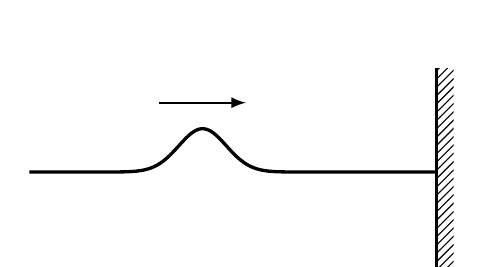
\begin{tikzpicture}[scale=1.1]
      \draw[very thick,smooth,samples=200,domain=-2:2.7]
      plot({\x},{.5*exp(-\x*\x/.15)});
      \draw[thick,->](-.5,.8)--(.5,.8);
      \draw[very thick](2.7,1.2)--(2.7,-1.2);
      \fill [pattern=north east lines] (2.7,1.2) rectangle(2.9,-1.2);
    \end{tikzpicture}
  }
  \question One end of a horizontal string is fixed to a wall. A transverse
  wave pulse is generated at the other end, moves toward the wall as shown
  above, and is reflected at the wall. Properties of the reflected pulse
  include which of the following?
  \begin{enumerate}[nosep,leftmargin=18pt,label={\Roman*.}]
  \item It has greater speed than that of the incident pulse.
  \item It has greater amplitude than that of the incident pulse.
  \item It is on the opposite side of the string from the incident pulse.
  \end{enumerate}
  \begin{choices}
    \choice I only
    \choice III only
    \choice I and II only
    \choice I and III only
    \choice I, II and III
  \end{choices}
  
  \uplevel{
    \vspace{-.25in}
    \pic{.4}{impulses}
  }
  \question\vspace{-.3in} Objects X and Y are constrained to move along a
  straight line. The
  graphs above show the net force exerted along that line on each of the
  objects as functions of time. Which of the following correctly ranks the
  change in momentum $\Delta p$ of the objects?
  \begin{choices}
    \choice $\Delta p_X < \Delta p_Y$
    \choice $\Delta p_X = \Delta p_Y$ 
    \choice $\Delta p_X > \Delta p_Y$
    \choice The ranking cannot be determined without knowing the masses\\
    of the objects.
  \end{choices}
    
  \question Three forces at on an object. If the object is in translational
  equilibrium, which of the following must be true?
  \begin{enumerate}[nosep,leftmargin=18pt,label={\Roman*.}]
  \item The vector sum of the three forces must be equal to zero
  \item The magnitudes of the three forces must be equal
  \item All three forces must be parallel
  \end{enumerate}
  \begin{choices}
    \choice I only
    \choice II only
    \choice I and III only
    \choice II and III only
    \choice I, II and III
  \end{choices}

  \uplevel{
    \pic{.6}{car-collision}
  }
  \question\vspace{-.2in}In the setup shown above, a student uses motion
  detector 1 to measure
  the speed $v_i$ of a cart with mass m before it collides with and sticks to
  a stationary cart with mass $M$. Motion detector 2 measures the speed $v_f$
  of the carts after the collision. The student repeats the experiment
  several times using different values of $v_i$ and creates a graph of $v_f$
  as a function of $v_i$. The slope of this graph is most nearly equal to
  \begin{choices}
    \choice$\dfrac mM$
    \choice$\dfrac{m}{M+m}$
    \choice$\dfrac{M-m}{M+m}$
    \choice$\sqrt{\dfrac{m}{M+m}}$
  \end{choices}
  
  \uplevel{
    \pic{.75}{circular-arc}
    \vspace{-.2in}\textbf{Questions \ref{first}--\ref{last}:} The figures above
    show a small block of mass \SI{.20}{\kilo\gram} on a track in the shape of
    a circular arc. The block is released from rest at a height $H$ above the
    floor, as shown in Figure 1. The block slides along the track with
    negligible friction and leaves it at a height of \SI{.40}{\metre} above the
    floor and a speed of \SI{3.}{\metre\per\second} at a \ang{30} angle, as
    shown in Figure 2.
  }

  \question The height $H$ is most nearly
  \begin{choices}
    \choice 0.45 m
    \choice 0.51 m
    \choice 0.86 m
    \choice 1.7 m
  \end{choices}
  \label{first}
    
  \question The magnitude of the gravitational force exerted on the block is
  $F_g$, and the magnitude of the normal force exerted by the track on the
  block is $F_n$. Which of the following correctly compares the magnitudes of
  these two forces when the block is at the lowest point on the track?
  \begin{choices}
    \choice $F_n>F_g$
    \choice $F_n=F_g$
    \choice $F_n<F_g$
    \choice The magnitudes cannot be compared without knowing the radius\\
    of the arc of the track.
  \end{choices}
    
  \question After the block leaves the track, what is the block's speed when it
  reaches the highest point of its motion?
  \begin{choices}
    \choice 0\hspace{.3in}
    \choice\SI{1.5}{\metre\per\second}\hspace{.3in} 
    \choice\SI{2.6}{\metre\per\second}\hspace{.3in}
    \choice\SI{3.0}{\metre\per\second}
  \end{choices}
  \label{last}
  
  \question Two satellites are in circular orbits around Earth. Satellite 1 has
  mass $m_0$ and an orbital radius of $2R_E$, where $R_E$ is the radius of
  Earth. Satellite 2 has mass $2m_0$ and an orbital radius of $3R_E$. Which of
  the following correctly compares the magnitude $F$ of the force exerted by
  Earth on each satellite and the speed $v$ of each satellite?

  \begin{tabular}{ccc}
    & Force & Speed\\ \hline
    (A) & $F_1>F_2$ & $v_1>v_2$ \\
    (B) & $F_1>F_2$ & $v_2>v_1$ \\
    (C) & $F_2>F_1$ & $v_1>v_2$ \\
    (D) & $F_2>F_1$ & $v_2>v_1$
  \end{tabular}    
  \newpage    

  \uplevel{
    \centering
    \begin{tikzpicture}[scale=1.3]
      \draw[very thick](0,0) rectangle(1,1);
      \draw[ultra thick,->](.5,-.75)--(.5,0) node[pos=0,below]{
        \begin{minipage}{\linewidth}
          \centering
          \small Force Exerted by Person\par
        \end{minipage}
      };
    \end{tikzpicture}
  }
  \question A person exerts an upward force on a box, as shown on the left. The
  box may be moving upward, downward, or not at all while the person exerts the
  upward force. For which of the following motions of the box is the work done
  by the person on the box correctly indicated?
  
  \begin{tabular}{clc}
    & Motion of Box & Work Done by Person on Box \\
    \hline
    (A) & No motion                  & Positive \\
    (B) & Upward, decreasing speed   & Negative \\
    (C) & Downward, constant speed   & Zero     \\
    (D) & Downward, increasing speed & Negative
  \end{tabular}

  \uplevel{
    \centering
    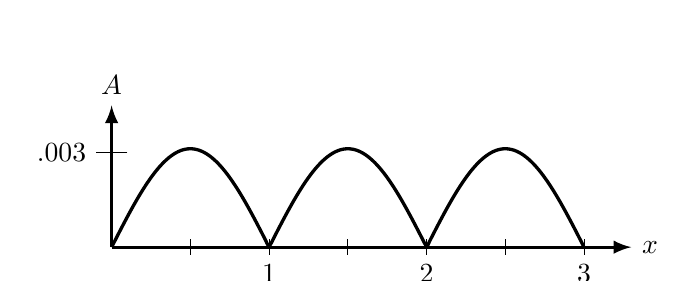
\begin{tikzpicture}[xscale=2]
      \draw[very thick,->](0,0)--(3.3,0) node[right]{$x$};
      \draw[very thick,->](0,0)--(0,1.8) node[above]{$A$};
      \foreach \x in {.5,1.5,2.5} \draw(\x,.1)--(\x,-.1);
      \foreach \x in {1,2,3} \draw(\x,.1)--(\x,-.1) node[below]{\x};
      \draw(.1,1.2)--(-.1,1.2) node[left]{.003};
      \draw[very thick,smooth,samples=200,domain=0:3]
      plot({\x},{1.25*abs(sin(180*\x))});
    \end{tikzpicture}
  }
  \question A standing wave is produced on a horizontal string of
  length \SI{3}{\metre} that is fixed at both ends. The graph above shows the
  amplitude $A$ of the vertical oscillations of points on the string as a
  function of the distance $x$ from one end of the string. For any point on the
  string, the amplitude is the absolute value of the maximum displacement of
  that point from its equilibrium position. The wavelength of the standing wave
  is
  \begin{choices}
    \choice 1.0 m
    \choice 1.5 m
    \choice 2.0 m
    \choice 3.0 m
  \end{choices}
  
  \uplevel{
    \pic{.27}{two-masses}
  }
  \question\vspace{-.2in} A block of mass \SI{3.}{\kilo\gram} is hung from a
  spring, causing it to stretch \SI{12}{\centi\metre} at equilibrium, as
  shown above. The \SI{3.}{\kilo\gram} block is then replaced by a
  \SI{4.}{\kilo\gram} block, and the new block is released from the positive
  shown above, at which the spring is unstretched. How far will the
  \SI{4.}{\kilo\gram} block fall before its direction is reversed?
  \begin{choices}
    \choice 9 cm
    \choice 18 cm
    \choice 24 cm
    \choice 32 cm
    \choice 48 cm
  \end{choices}
    
%  \question Which of the following statements about a satellite in an elliptical
%    orbit around Earth are correct? Select two answers.
%    \begin{choices}
%    \choice The satellite's kinetic energy is constant throughout the orbit.
%    \choice The satellite's angular momentum about the center of mass of the
%      satellite-Earth system is constant throughout the orbit.
%    \choice The magnitude of the satellite's linear momentum is constant
%      throughout the orbit.
%    \choice The gravitational potential energy of the Earth-satellite system is
%      greatest at the satellite's farthest point from Earth.
%    \end{choices}
%    \vspace{.7in}
    
  \question Which of the following can be used as evidence for the claim that
  the energy carried by a mechanical wave increases with the amplitude of the
  wave?
  \begin{choices}
    \choice A person does not move when a small ocean wave passes by but is
    pushed over by a higher wave.
    \choice A high-pitched sound may cause more discomfort to a person's ear
    than a low-pitched sound does.
    \choice The interference of two waves of amplitude $A_0$ may result in an
    amplitude that is either larger or smaller than $A_0$.
    \choice A wave pulse on a string is larger or smaller, depending on how far
    the person creating the pulse moves the end of the string.
  \end{choices}
  \vspace{.5in}
  
  \uplevel{
    \centering
    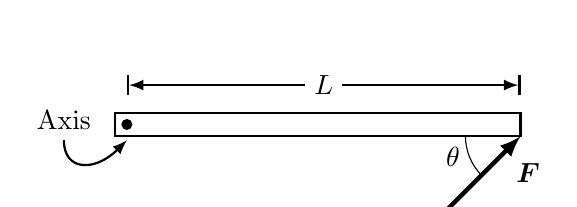
\begin{tikzpicture}
      \fill(0,0) circle(.07);
      \draw[thick](-.15,-.15) rectangle(5,.15);
      \draw[thick,|<->|](0,.5)--(5,.5) node[midway,fill=white]{$L$};
      \draw[ultra thick,->](4,-1.15)--(5,-.15)
      node[pos=.8,below right]{$\bm{F}$};
      \draw(4.3,-.15) arc(180:225:.7) node[midway,left]{$\theta$};
      \draw[thick,->] (-.8,-.2)..controls(-.8,-.6) and (-.4,-.6)..(0,-.2)
      node[pos=0,above]{Axis};
    \end{tikzpicture}
    
      View from Above
  }
  \question A rod on a horizontal tabletop is pivoted at one end and is free to
  rotate without friction about a vertical axis, as shown above. A force
  $\bm{F}$ is applied at the other end, at an angle $\theta$ to the rod. If
  $\bm{F}$ were to be applied perpendicular to the rod, at what distance from
  the axis should it be applied in order to produce the same torque?
  \begin{choices}
    \choice$L\sin\theta$
    \choice$L\cos\theta$
    \choice$L$
    \choice$L\tan\theta$
    \choice$\sqrt{2}L$
  \end{choices}
  \newpage
  
  \uplevel{
    \centering
    \begin{tikzpicture}[scale=1.8]
      \draw[thick,->](0,0)--(0,1)node[midway,left]{$mV$};
      \draw[thick,->](0,0)--(1,0)node[midway,below]{$mV$};
    \end{tikzpicture}
  }
  \question A stationary object explodes, breaking into three pieces of masses
  $m$, $m$ and $3m$. The two pieces of mass $m$ move off at right angles to each
  other with the same magnitude of momentum $mV$, as shown in the diagram
  above. What are the magnitude and direction of the velocity of the piece
  having mass $3m$?

  \begin{tabular}{ccc}
    & Magnitude & Direction \\
    \hline
    (A) & $\dfrac{V}{\sqrt{3}}$  & {\Huge $\nearrow$} \\
    (B) & $\dfrac{V}{\sqrt{3}}$  & {\Huge $\swarrow$} \\
    (C) & $\dfrac{\sqrt{2}V}{3}$ & {\Huge $\nearrow$} \\
    (D) & $\dfrac{\sqrt{2}V}{3}$ & {\Huge $\swarrow$} \\
    (E) & $\sqrt{2}V$ & {\Huge $\swarrow$}
  \end{tabular}
    
  \question An old record player could bring a disk up to 45 rpm speed in less
  than a second. If the same size disk can also be brought up to a speed of 75
  rpm in about the same amount of time on another player, compare the two
  torques.
  \begin{choices}
    \choice The torques would be the same as the amount of rotational inertia of
    the two disks are the same.
    \choice The torques would be the same because of the conservation of angular
    momentum.
    \choice The torque would be larger in the second case as it requires a
    greater angular acceleration.
    \choice The torque would be larger in the second case as it entails both a
    larger force and a larger lever arm.
  \end{choices}

  \uplevel{
    \centering
    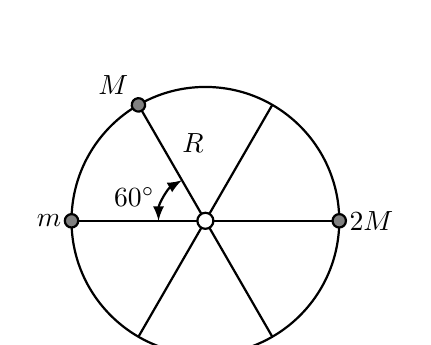
\begin{tikzpicture}[scale=1.7]
      \begin{scope}[thick]
        \draw (0,0) circle(1);
        \draw (-1,0)--(1,0);
        \draw[fill=gray](-1,0) circle(.05) node[left]{$m$};
        \draw[fill=gray]( 1,0) circle(.05) node[right]{$2M$};
        \draw[rotate=60](-1,0)--(1,0);
        \begin{scope}[rotate=-60]
          \draw (-1,0)--(1,0) node[pos=.25,above right]{$R$};
          \draw[fill=gray](-1,0) circle(.05) node[above left]{$M$};
        \end{scope}
        \draw[<->](-.35,0) arc(180:120:.35) node[midway,left]{\ang{60}};
        \draw[fill=white](0,0) circle(.06);
      \end{scope}
    \end{tikzpicture}
  }
  \question A wheel of radius $R$ and negligible mass is mounted on a horizontal
  frictionless axle so that the wheel is in a vertical plane. Three small
  objects having masses $m$, $M$ and $2M$, respectively, are mounted on the
  rim of the wheel, as shown above. If the system is in static equilibrium,
  what is the value of $m$ in terms of $M$?
  \begin{choices}
    \choice$\dfrac M2$
    \choice$M$
    \choice$\dfrac{3M}2$
    \choice$2M$
    \choice$\dfrac{5M}2$
  \end{choices}
  
  \question A \SI{2}{\kilo\gram} object moves in a circle of radius
  \SI4{\metre} at a constant speed of \SI3{\metre\per\second}. A net force of
  \SI{4.5}{\newton} acts on the object. What is the angular momentum of the
  object with respect to an axis perpendicular the circle and through its
  center?
  \begin{choices}
    \choice\SI{9}{N.m/kg}
    \choice\SI{12}{m^2/s}
    \choice\SI{13.5}{kg.m^2/s^2}
    \choice\SI{18}{N.m/kg}
    \choice\SI{24}{kg.m^2/s}
  \end{choices}
  
  \uplevel{
    \centering
    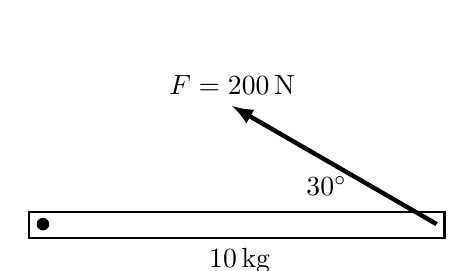
\begin{tikzpicture}
      \fill(-5,0) circle(.08);
      \draw[thick](-5.18,-.18) rectangle (.1,.15);
      \node[below] at (-2.5,-.18){\SI{10}{\kilo\gram}};
      \draw[ultra thick,->,rotate=-30](0,0)--(-3,0)
      node[midway,below]{\ang{30}\;\;}
      node[above]{$F=\SI{200}{\newton}$};
    \end{tikzpicture}
  }
    
  \question What is the net torque acting on the pivot supporting a
  \SI{10}{\kilo\gram} beam 2 meters long as shown above?
  \begin{choices}
    \choice\SI{198}{\newton\metre}
    \choice\SI{-198}{\newton\metre}
    \choice\SI{-102}{\newton\metre}
    \choice\SI{102}{\newton\metre}
  \end{choices}
  \newpage  

  \uplevel{
    \textbf{Questions \ref{mass1}--\ref{mass2}:} A \SI{.4}{\kilo\gram} mass is
    oscillating on a spring that has a force constant of
    $k=\SI{1000}{\newton\per\metre}$.
  }

  \question Which of the following measurements would allow you to determine the
  maximum velocity experienced by the mass?
  \label{mass1}
  \begin{choices}
    \choice No additional information is required.
    \choice Minimum velocity
    \choice Maximum acceleration
    \choice None of these would allow you to determine maximum velocity
  \end{choices}
    
  \question Which of the following statements concerning the oscillatory motion
  described is correct? (All statements refer to magnitudes.)
  \label{mass2}
  \begin{choices}
    \choice The maximum velocity and maximum acceleration occurs at the same
    time.
    \choice The maximum velocity occurs when the acceleration is a minimum.
    \choice The velocity is always directly proportional to the displacement.
    \choice The maximum velocity occurs when the displacement is a maximum.
  \end{choices}

  \uplevel{
    \pic{.25}{disks}
  }
  \question Cylindrical disk $A$ is rotating freely about an axis when an
  identical disk $B$ that is not rotating is dropped directly on top of disk
  $A$. If the two disks stick together, how does the total angular momentum
  and total kinetic energy of the two-disk system after the disks are stuck
  together compare to that of the system before disk $B$ was dropped?
  
  \begin{tabular}{cll}
    & Total Angular Momentum & Total Kinetic Energy\\
    \hline
    (A) & Remains the same & $\dfrac12$ its original value\\
    (B) & Remains the same & $\dfrac14$ its original value\\
    (C) & $\dfrac12$ its original value & $\dfrac12$ its original value\\
    (D) & $\dfrac12$ its original value & $\dfrac14$ its original value
  \end{tabular}
\end{questions}

%\vspace{\stretch{1}}
%\begin{center}
%  \textbf{\LARGE S T O P}
%  
%  \vspace{.3in}END OF SECTION I
%
%  \vspace{.3in}IF YOU FINISH BEFORE TIME IS CALLED, YOU MAY\\
%  CHECK YOUR WORK ON THIS SECTION
%
%  \vspace{.3in}DO NOT GO ON TO SECTION II UNTIL YOU ARE TOLD TO DO SO
%\end{center}
\end{document}
